\documentclass[10pt,oneside,english]{lips}

%\usepackage[square]{natbib}\bibliographystyle{plainnat}\setcitestyle{numbers}
\usepackage[round]{natbib}\bibliographystyle{plainnat}

% Configure the document
\title{Requirement specification}
\author{Editor name}
\date{November 1 2015}
\version{1.0}

\reviewed{Ewa, Karl}{2015-xx-xx}
\approved{Moa}{2015-xx-xx}

\projecttitle{Title of an inspiring project}

\groupname{Group name}
\groupemail{groupmail@liu.se}
\groupwww{http://www.isy.liu.se/tsrt10/group}

\coursecode{TSRT10}
\coursename{Control theory project course}

\orderer{Orderer, Linköpings universitet}
\ordererphone{+46 xxxxxx}
\ordereremail{ordere@liu.se}

\customer{Customer, Company X}
\customerphone{+46 xxxxxx}
\customeremail{customer@companyx.com}

\courseresponsible{Boss Person}
\courseresponsiblephone{+46 xxxxxx}
\courseresponsibleemail{the.boss@liu.se}

\supervisor{Supervisor}
\supervisorphone{+46 xxxxxx}
\supervisoremail{super.visor@liu.se}

\smalllogo{logo} % Page header logo, filename
\biglogo{logo} % Front page logo, filename

\cfoot{\thepage}
\begin{document}
\maketitle

\cleardoublepage
\makeprojectid

\begin{center}
  \Large Participants of the group
\end{center}
\begin{center}
  \begin{tabular}{|l|l|l|}
    \hline
    \textbf{Name} & \textbf{Responsible} & \textbf{E-mail}\\
    \hline
    Anna Andersson & Responsible for customer relations (CUS) & Annan111@student.liu.se\\
    \hline
    Beata Bson & Responsible for the Documentation (DOC) & Beabs222@student.liu.se\\
    \hline
    Cecilia Cson & Responsible for the design (DES) & Ceccs333@student.liu.se\\
    \hline
    Doris Dson & Responsible for the testing (TEST) & Dords444@student.liu.se\\
    \hline
    Erik Eson & Responsible for the quality (QA) & Eries555@student.liu.se\\
    \hline
    Fredrik Fson & Responsible for the implementation (IMP) & Frefs666@student.liu.se\\
    \hline
    Greta Gson & Project leader (PL) & Gregs777@student.liu.se\\
    \hline
  \end{tabular}
\end{center}

\cleardoublepage
\tableofcontents

\cleardoublepage
\section*{Document History}
\begin{tabular}{p{.06\textwidth}|p{.1\textwidth}|p{.45\textwidth}|p{.13\textwidth}|p{.13\textwidth}} 
  \multicolumn{1}{c}{\bfseries Version} & 
  \multicolumn{1}{|c}{\bfseries Date} & 
  \multicolumn{1}{|c}{\bfseries Changes made} & 
  \multicolumn{1}{|c}{\bfseries Sign} & 
  \multicolumn{1}{|c}{\bfseries Reviewer}\\
  \hline
  \hline
  0.1 & 2015-11-01 & First draft. & Sign1 & Name1   \\
  \hline
  0.2 & 2015-11-03 & First revision & Sign2 & Name2   \\
  \hline
\end{tabular}

\cleardoublepage
\pagenumbering{arabic}\cfoot{\thepage}

\section{Introduction}
\label{sec:inledning}

Text
\begin{figure}[htbp]
  \centering
  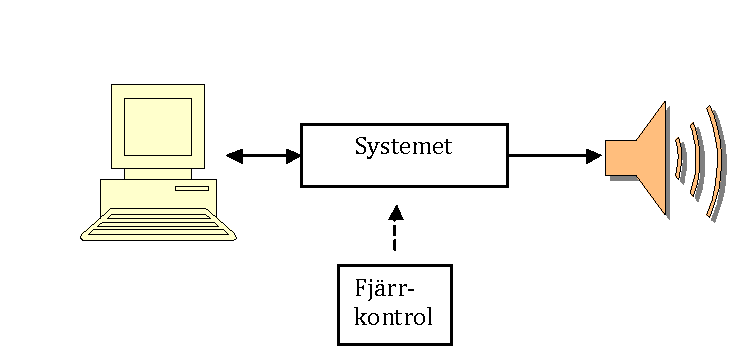
\includegraphics[width=.7\textwidth]{sys}
  \caption{The system in its surroundings}
  \label{fig:sys}
\end{figure}

\begin{requirements}
  \requirementno & All documents shall follow instructions in \citep{spraknamnd:2000} & 1\\
\end{requirements}

\subsection{Partners}
Text

\subsection{Aims and goals}
Text

\subsection{Use}
Text

\subsection{Background information}
Text

\subsection{Definition of terms}
Text

\section{System overview}
Text
\begin{figure}[htbp]
  \centering
  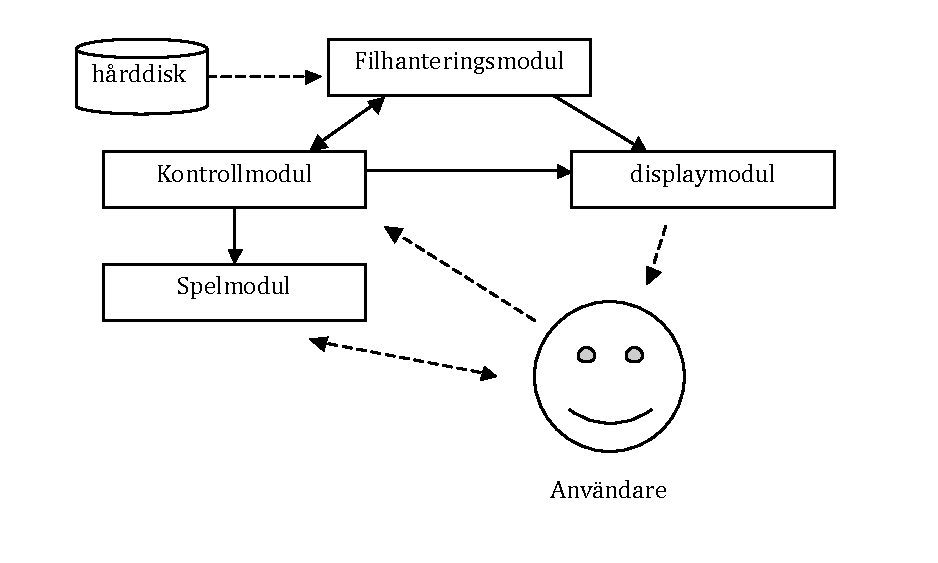
\includegraphics[width=.7\textwidth]{outline}
  \caption{An overview of the system.}
  \label{fig:oversikt}
\end{figure}

\subsection{Description of the product}
Text

\subsection{Product components}
Text

\subsection{Dependency of other systems}
Text

\subsection{Included sub-systems}
Text

\subsection{Limitations}
Text

\subsection{Design philosophy}
Text

\section{Subsystem 1}
Text
\begin{figure}[htbp]
  \centering
  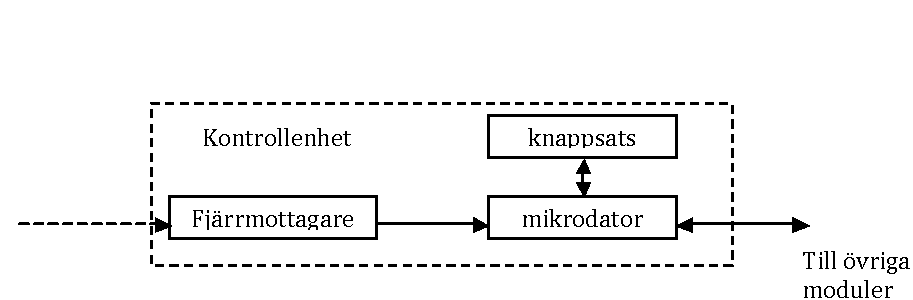
\includegraphics[width=.7\textwidth]{delsys1}
  \caption{Subsystem 1.}
  \label{fig:delsys1}
\end{figure}

\subsection{Introductory description of sub-system 1}
Text
\begin{requirements}
  \requirementno & Error messages must be in English & 1\\
\end{requirements}

\subsection{Interfaces}
\begin{requirements}
  \requirementno\label{req:r2} & Text of requirement & Expired\\
  \ref{req:r2}A & New text for requirement \ref{req:r2} & 1\\
\end{requirements}
Text

\subsection{Design requirements}
Text
\begin{requirements}
  \requirementno & Text for requirement & 2\\
  \requirementno & Text for requirement & 3\\
\end{requirements}

\subsection{Functional requirements}
Text
\begin{requirements}
  \requirementno & Text for requirement & 2\\
  \requirementno & Text for requirement & 3\\
\end{requirements}

\section{Subsystem 2}
Text
\begin{figure}[htbp]
  \centering
  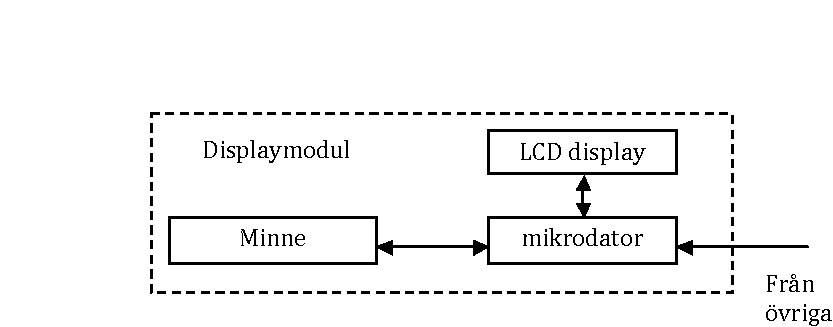
\includegraphics[width=.7\textwidth]{delsys2}
  \caption{Subsystem 2}
  \label{fig:delsys2}
\end{figure}

\subsection{External interfaces}
Text
\begin{requirements}
  \requirementno & Text for requirement & 3\\
\end{requirements}

\subsection{Design requirements}
Text
\begin{requirements}
  \requirementno & Text for requirement & 3\\
\end{requirements}


\subsection{Functional requirements for subsystem 2}
Text
\begin{requirements}
  \requirementno & Text for requirement & 1\\
  \requirementno & One more requirement & 3\\
\end{requirements}

\subsection{User interface}
Text
\begin{requirements}
  \requirementno & Text for requirement & 3\\
\end{requirements}

\section{Performance requirements}
Text
\begin{requirements}
  \requirementno & Text for requirement & 1\\
\end{requirements}

\section{Possibilities to upgrade}
Text
\begin{requirements}
  \requirementno & Text for requirement & 1\\
\end{requirements}

\section{Reliability}
Text
\begin{requirements}
  \requirementno & Text for requirement & 1\\
\end{requirements}

\section{Economy} 
Text
\begin{requirements}
  \requirementno & Text for requirement & 1\\
\end{requirements}

\section{Safety and security requirements}
Text
\begin{requirements}
  \requirementno & Text for requirement & 1\\
\end{requirements}

\section{Delivery} 
Text
\begin{requirements}
  \requirementno & Text for requirement & 1\\
\end{requirements}

\section{Documentation} 
Table~\ref{tab:doks} lists all documents that shall be produced in the
project
\begin{table}[htbp]
  \centering
  \caption{Documents to be produced.}
  \label{tab:doks}
  \begin{tabular}{|l|l|l|l|l|}
    \hline
    Document & Language & Aim & Target & Format\\
    \hline
    Project plan &&&&\\
    Requirement specification &&&&\\
    Design specifikation &&&&\\
    Meeting minutes &&&&\\
    Technical documentation &&&&\\
    After study &&&&\\
    \hline
  \end{tabular}  
\end{table}

\section{Training}
Text
\begin{requirements}
  \requirementno & Text for requirement & 1\\
\end{requirements}

\section{Quality}
Text
\begin{requirements}
  \requirementno & Text for requirement & 1\\
\end{requirements}

\section{Maintainability}
Text
\begin{requirements}
  \requirementno & Text for requirement & 1\\
\end{requirements}


\clearpage
\bibliography{references}

\cleardoublepage
\appendix

\section{Appendix title}

\subsection{The first heading}
Text

\subsubsection{First sub-heading}
Text

\subsubsection{Second sub-heading}
Text

\subsubsection{Third sub-heading}
Text

\end{document}

%%% Local Variables:
%%% mode: latex
%%% TeX-master: t
%%% End:
